\appendix

\chapter{Additional Experimental Figures}
\label{app:additional_experimental_figures}

This appendix contains large experimental figures that are required for evaluation but are not
legible at the standard inline size used in the main chapters. They are referenced from
Chapter~\ref{chap:experiments} where their corresponding results are discussed.

\section{Large Confusion Matrix}
\label{app:large_confusion_matrix}

Figure~\ref{fig:app_cm_msasl50} shows the row-normalised confusion matrix for the MS-ASL50
seed-2026 run. The matrix is placed here because the 50-class layout requires a full page to make
the class labels and off-diagonal errors readable.

\begin{figure}[p]
    \centering
    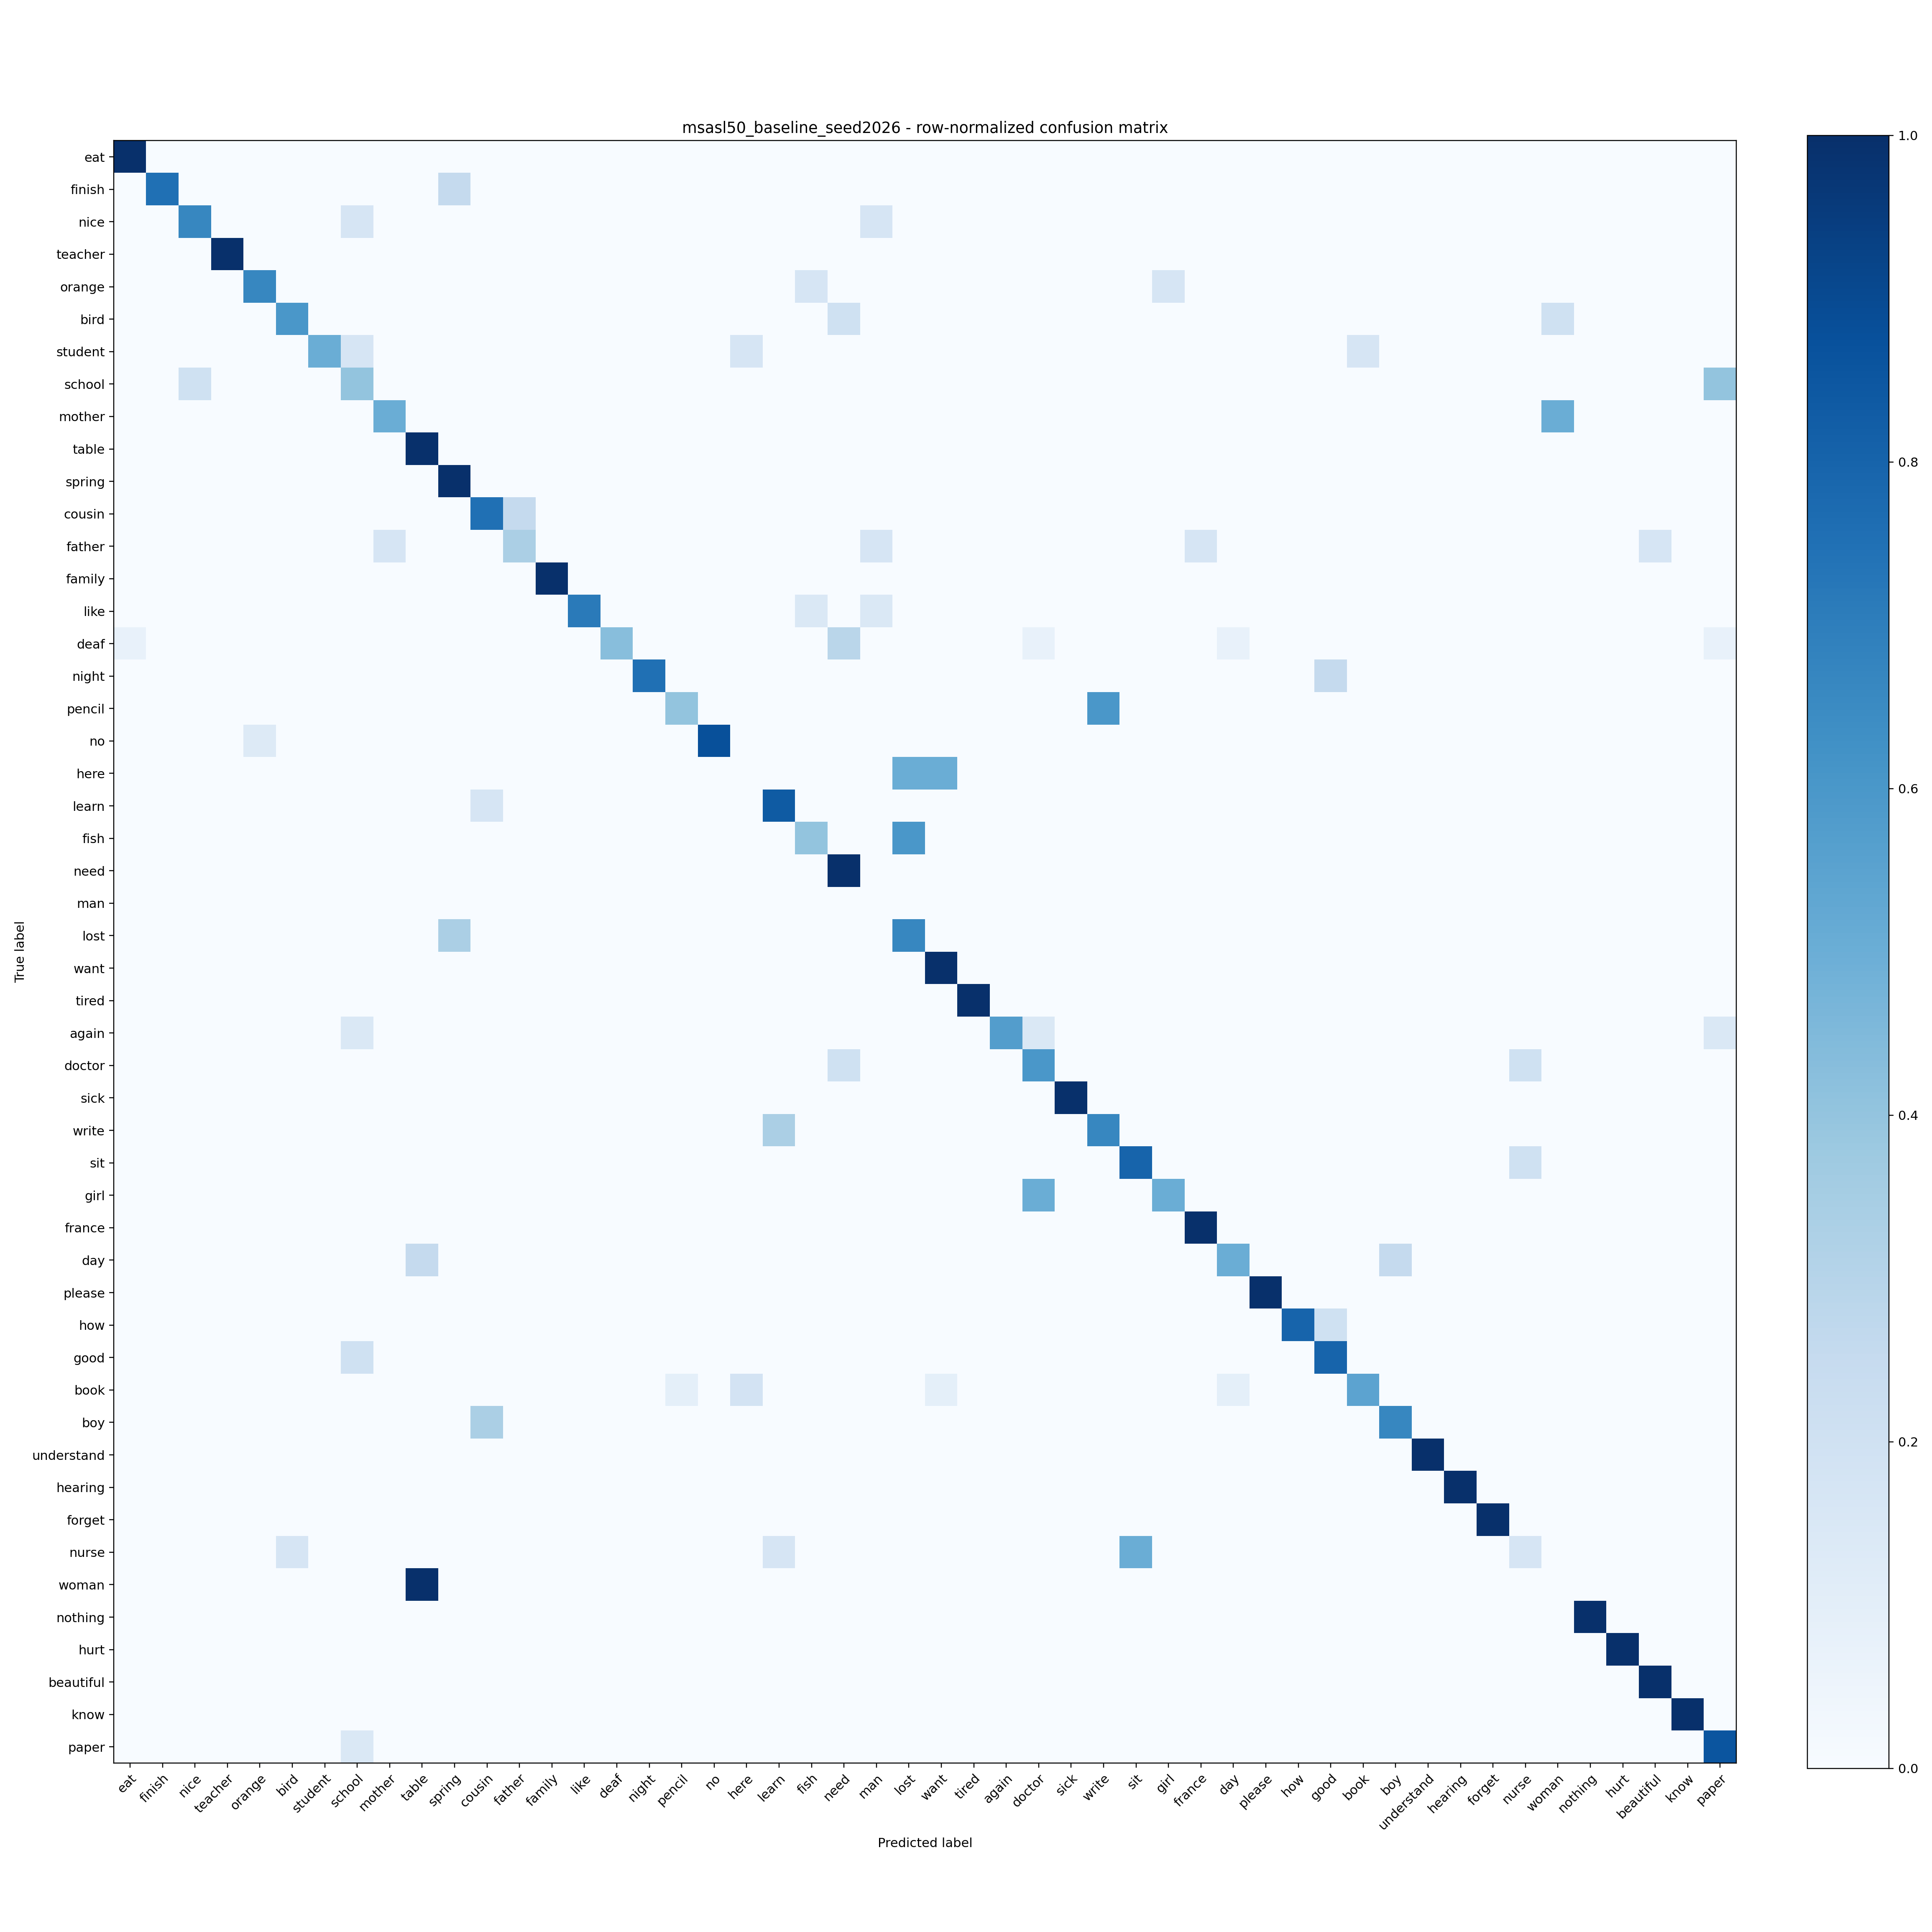
\includegraphics[width=\textwidth,height=0.82\textheight,keepaspectratio]{./images/results/confusion_matrix_msasl50_seed2026.png}
    \caption{Row-normalised confusion matrix on the MS-ASL50 test split for seed 2026 (236 samples). Source: self-created from experiment outputs.}
    \label{fig:app_cm_msasl50}
\end{figure}

\clearpage

\section{Vocabulary Scaling Diagnostic}
\label{app:vocabulary_scaling_diagnostic}

Figure~\ref{fig:app_scaling_parallel} shows the parallel-coordinates diagnostic used in
Section~\ref{sec:exp_scaling}. Each line corresponds to one vocabulary-scaling run, projected onto
mean videos per class, final train accuracy, validation Top-1, test Top-1 and test Top-5.

\begin{landscape}
\begin{figure}[p]
    \thispagestyle{empty}
    \centering
    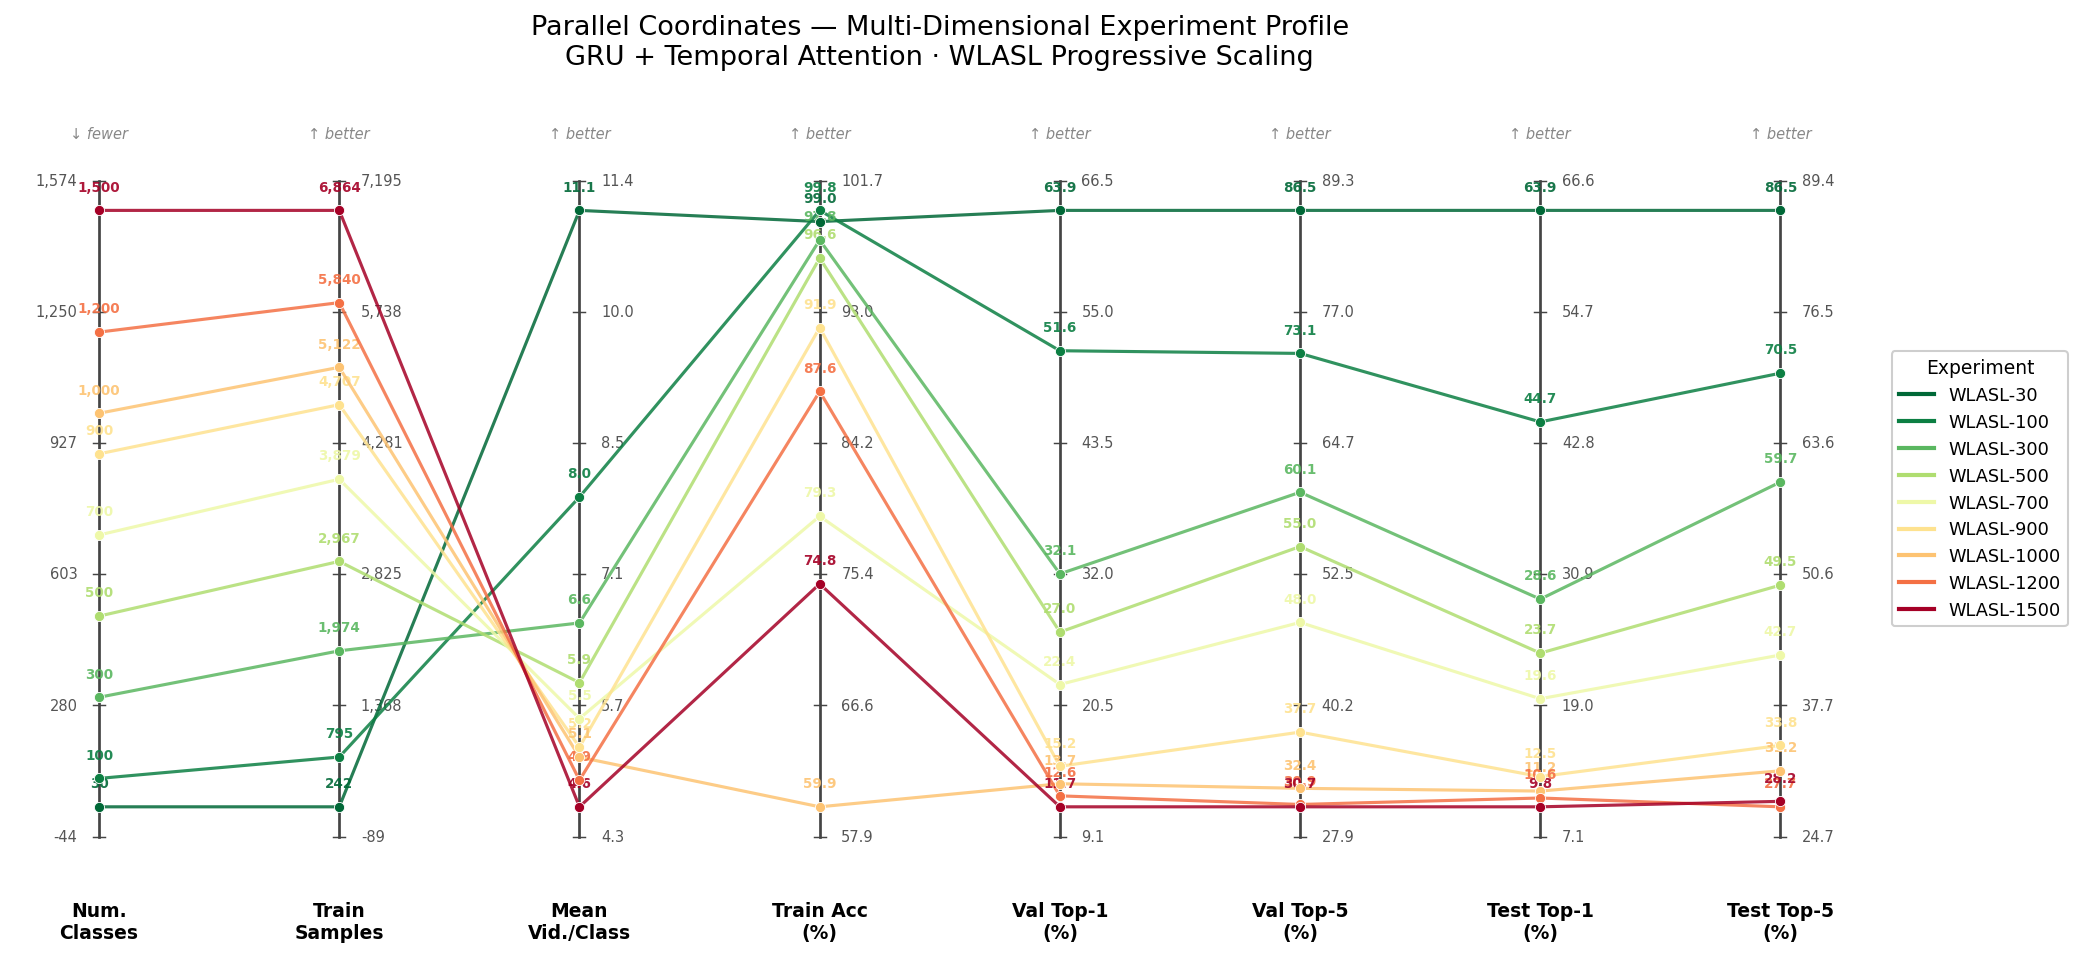
\includegraphics[width=\linewidth,height=0.82\textheight,keepaspectratio]{./images/results/scaling_parallel_coordinates.png}
    \caption{Parallel-coordinates view of the selected GRU+Attention scaling line on WLASL. Each line is one experiment, coloured from green for smaller vocabularies to red for larger vocabularies. Source: self-created from experiment outputs.}
    \label{fig:app_scaling_parallel}
\end{figure}
\end{landscape}
